\documentclass[12pt,a4paper,titlepage]{report}
\special{papersize=210mm,297mm}
\usepackage[italian]{babel}
\usepackage{amsmath, amsfonts, amssymb, mathrsfs, dsfont}
\usepackage[utf8]{inputenc}
\usepackage{fancyhdr}
\usepackage{fullpage}
\usepackage{color}
\usepackage{graphicx}
\pagestyle{fancy}
\begin{document}
\subsection{Formatura CR-RC}
Se io combino i due filtri precedentemente descritti frapponendo fra i due un amplificatore operazionale (fig~\ref{fig:filtroCRRC}) con guadagno pari a 1,
si ottiene una catena di lettura in grado di formare sia il fronte di salita che il fronte di discesa dell'impulso.
\begin{figure}[htbp]
\begin{center}
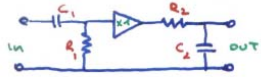
\includegraphics[scale=1]{FiltroCRRC.png}
\caption{Formatura tramite un CR-RC}
\label{fig:filtroCRRC}
\end{center}
\end{figure}
Se supponiamo di sottoporre la catena ad un gradino di tensione di ampiezza $V_0$ (approssima bene i segnali in uscita da un preamplificatore), in uscita si otterr\`a:
\begin{equation*}
V(t) = V_0 \, e^{-t/\tau_2}(1 - e^{-t/\tau_1}) 
\end{equation*}
Se $\tau_1 \approx \tau_2$ e sviluppando al primo ordine il termine tra parentesi si ottiene:
\begin{equation*}
V(t) = V_0 \, e^{-t / \tau} \frac{t}{\tau}
\end{equation*}
Il tempo caratteristico del RC (passa basso) determina il fronte di salita: aumentando $\tau$ (=$RC$) aumenta la frequenza di taglio, per cui passando le frequenze pi\`u alte aumentando la velocit\`a di salita.
Il tempo caratteristico del CR (passa alto) determina il fronte di discesa: se $\tau$ diminuisce la frequenza di taglio cala, di conseguenza le frequenze pi\`u alte vengono smorzate, diminuendo il tempo di discesa.
In conclusione aumentare $\tau_{RC}$ aumenta la velocit\`a di salita, aumentare $\tau_{CR}$ diminuisce la velocit\`a di discesa.\\
Le costanti di tempo devono essere scelte in modo tale da poter raccogliere le cariche disponibili, ridurre il rumore elettronico ed evitare il \textit{pile-up}.
In particolare alcune richieste sono in contrapposizione, ad esempio per essere sicuri di raccogliere tutte le cariche pu\`o essere utile avere un tempo di discesa lungo, 
tuttavia questo aumenta il rischio di avere del \textit{pile-up}. 
\begin{figure}[htbp]
\begin{center}
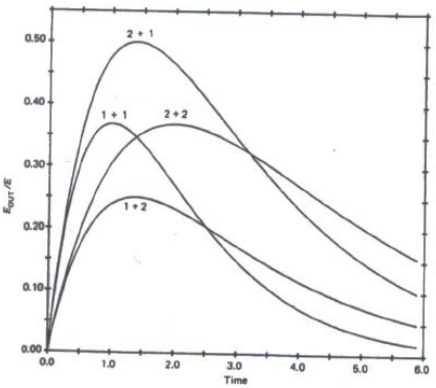
\includegraphics[scale=1]{FormaturaRCCR.png}
\caption{Esempi di segnali formati con varie costanti di tempo}
\label{fig:formaturaRCCR}
\end{center}
\end{figure}
\subsection{Formatura gaussiana}
Costruendo un circuito CR-(RC)$^n$ con n RC in cascata si pu\`o ottenere una formatura gaussiana dell'impulso:
\begin{equation}
V(t) = V_0 \, e^{-t/\tau} (1-e^{-t/\tau})^n \approx V_0 \left(\frac{t}{\tau}\right)^n e^{-t/\tau}
\end{equation}
Questa forma per $n>4$ approssima bene una gaussiana;
il massimo viene raggiunto in $n\tau$, detto anche \textit{\textbf{peaking time}}).
A parit\`a di \textit{peaking time}, questa formatura recupera la linea di base pi\`u velocemente rispetto alla formatura RC-CR.
Questa formatura \`e la migliore in qualit\`a di rapporto segnale-rumore.
\subsection{Formature con fitri attivi}
Utilizzando circuiti con elementi attivi come diodi o transistor si possono ottenere formature pi\`u fantasiose.
\begin{itemize}
\item \textbf{Formatura triangolare}, ottenibile con una serie di filtri attivi
\item \textbf{Formatura trapezoidale}, utilizzata se il risetime \`e variabile, in modo da avere tutta la carica raccolta in rivelatori con grande variabilit\`a di tempi di risposta.
Questa formatura viene ottenuta con circuiti analogici e digitali.
\end{itemize}
\subsection{Formatura CR-RC-CR}
Utilizzata per dare una forma bipolare all'impulso nel caso di rate molto elevati.
\subsection{Formatura con singola linea di ritardo}
La singola linea di ritardo (SDL) viene utilizzata per ridurre la durata di impulsi troppo lunghi:
un segnale viene sdoppiato in due rami, uno \`e il ramo di output, l'altro viene lasciato aperto.
Se il tempo di propagazione $\tau$ in quest'ultimo \`e molto maggiore del tempo di salita dell'impulso, allora dopo $2 \tau$ il segnale ritorna sulla linea di output, 
ma invertito.
Sommandosi al segnale precedente lo annulla.
\begin{figure}[htbp]
\begin{center}
	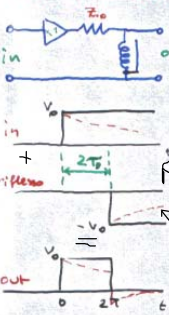
\includegraphics[scale=1]{SDL.png}
	\caption{Formatura con SDL (Single Delay Line)}
\label{fig:SDL}
\end{center}
\end{figure}
Nel caso il segnale avesse un decadimento si pu\`o presentare il problema dell'\textit{undershoot} (tratteggio rosso nell'immagine): per risolverlo
\`e necessario attenuare in modo opportuno il segnale.
\subsection{Formatura con doppia linea di ritardo}
\`E possibile rendere il segnale bipolare imponendo un altra linea di ritardo in uscita dalla SDL con lo stesso tempo della prima linea.
Il problema di questa formatura \`e che non passa da filtri, per cui presenta il problema del rumore non filtrato, per questo viene usata prevalentemente
in rivelatori con poca risoluzione o per i segnali logici.
\section{Cancellazione del polo zero}
Nella realt\`a i nostri dispositivi non sono sottoposti a dei gradini, bensi a segnali che salgono molto velocemente e decadono molto lentamente.
I tempi di decadimento possono portare a degli \textit{undershoot} che vengono recuperati in tempi nell'ordine dei $\mu$s causando problemi nella forma degli
impulsi successivi. \\
Si dimostra che nei CR-RC il problema pu\`o essere risolto utilizzando una resistenza regolabile in parallelo alla capacit\`a nel CR.
\section{Spostamenti della linea di base}
Supponiamo di avere un treno di impulsi, poich\`e in un CR-RC la tensione media deve essere nulla, in caso di alti rate si pu\`o osservare uno spostamento
della linea di base in modo da mantenere tale media nulla.\\
Nel caso di impulsi identici equispaziati lo spostamento non \`e problematico in quanto costante, tuttavia nella realt\`a gli impulsi hanno forma diversa per cui lo spostamento
pu\`o risultare un problema.\\
Per risolvere il problema si pu\`o usare una formatura bipolare in modo da compensare questo effetto, tuttavia porta ad avere alti rapporti rumore-segnale.
Un'altra soluzione proviene dall'accoppiare il segnale in tensione continua che successivamente viene eliminato con un filtro.



\end{document}